\section{Tempora}
\subsection{}

\begin{frame}
    \frametitle{Tempora}
    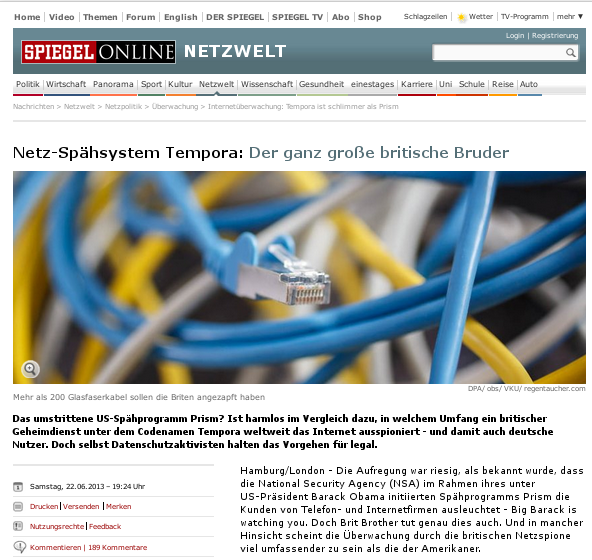
\includegraphics[height=0.7\textheight]{img/spiegel-tempora.png}
\end{frame}

\begin{frame}
    \frametitle{Kindernet}
    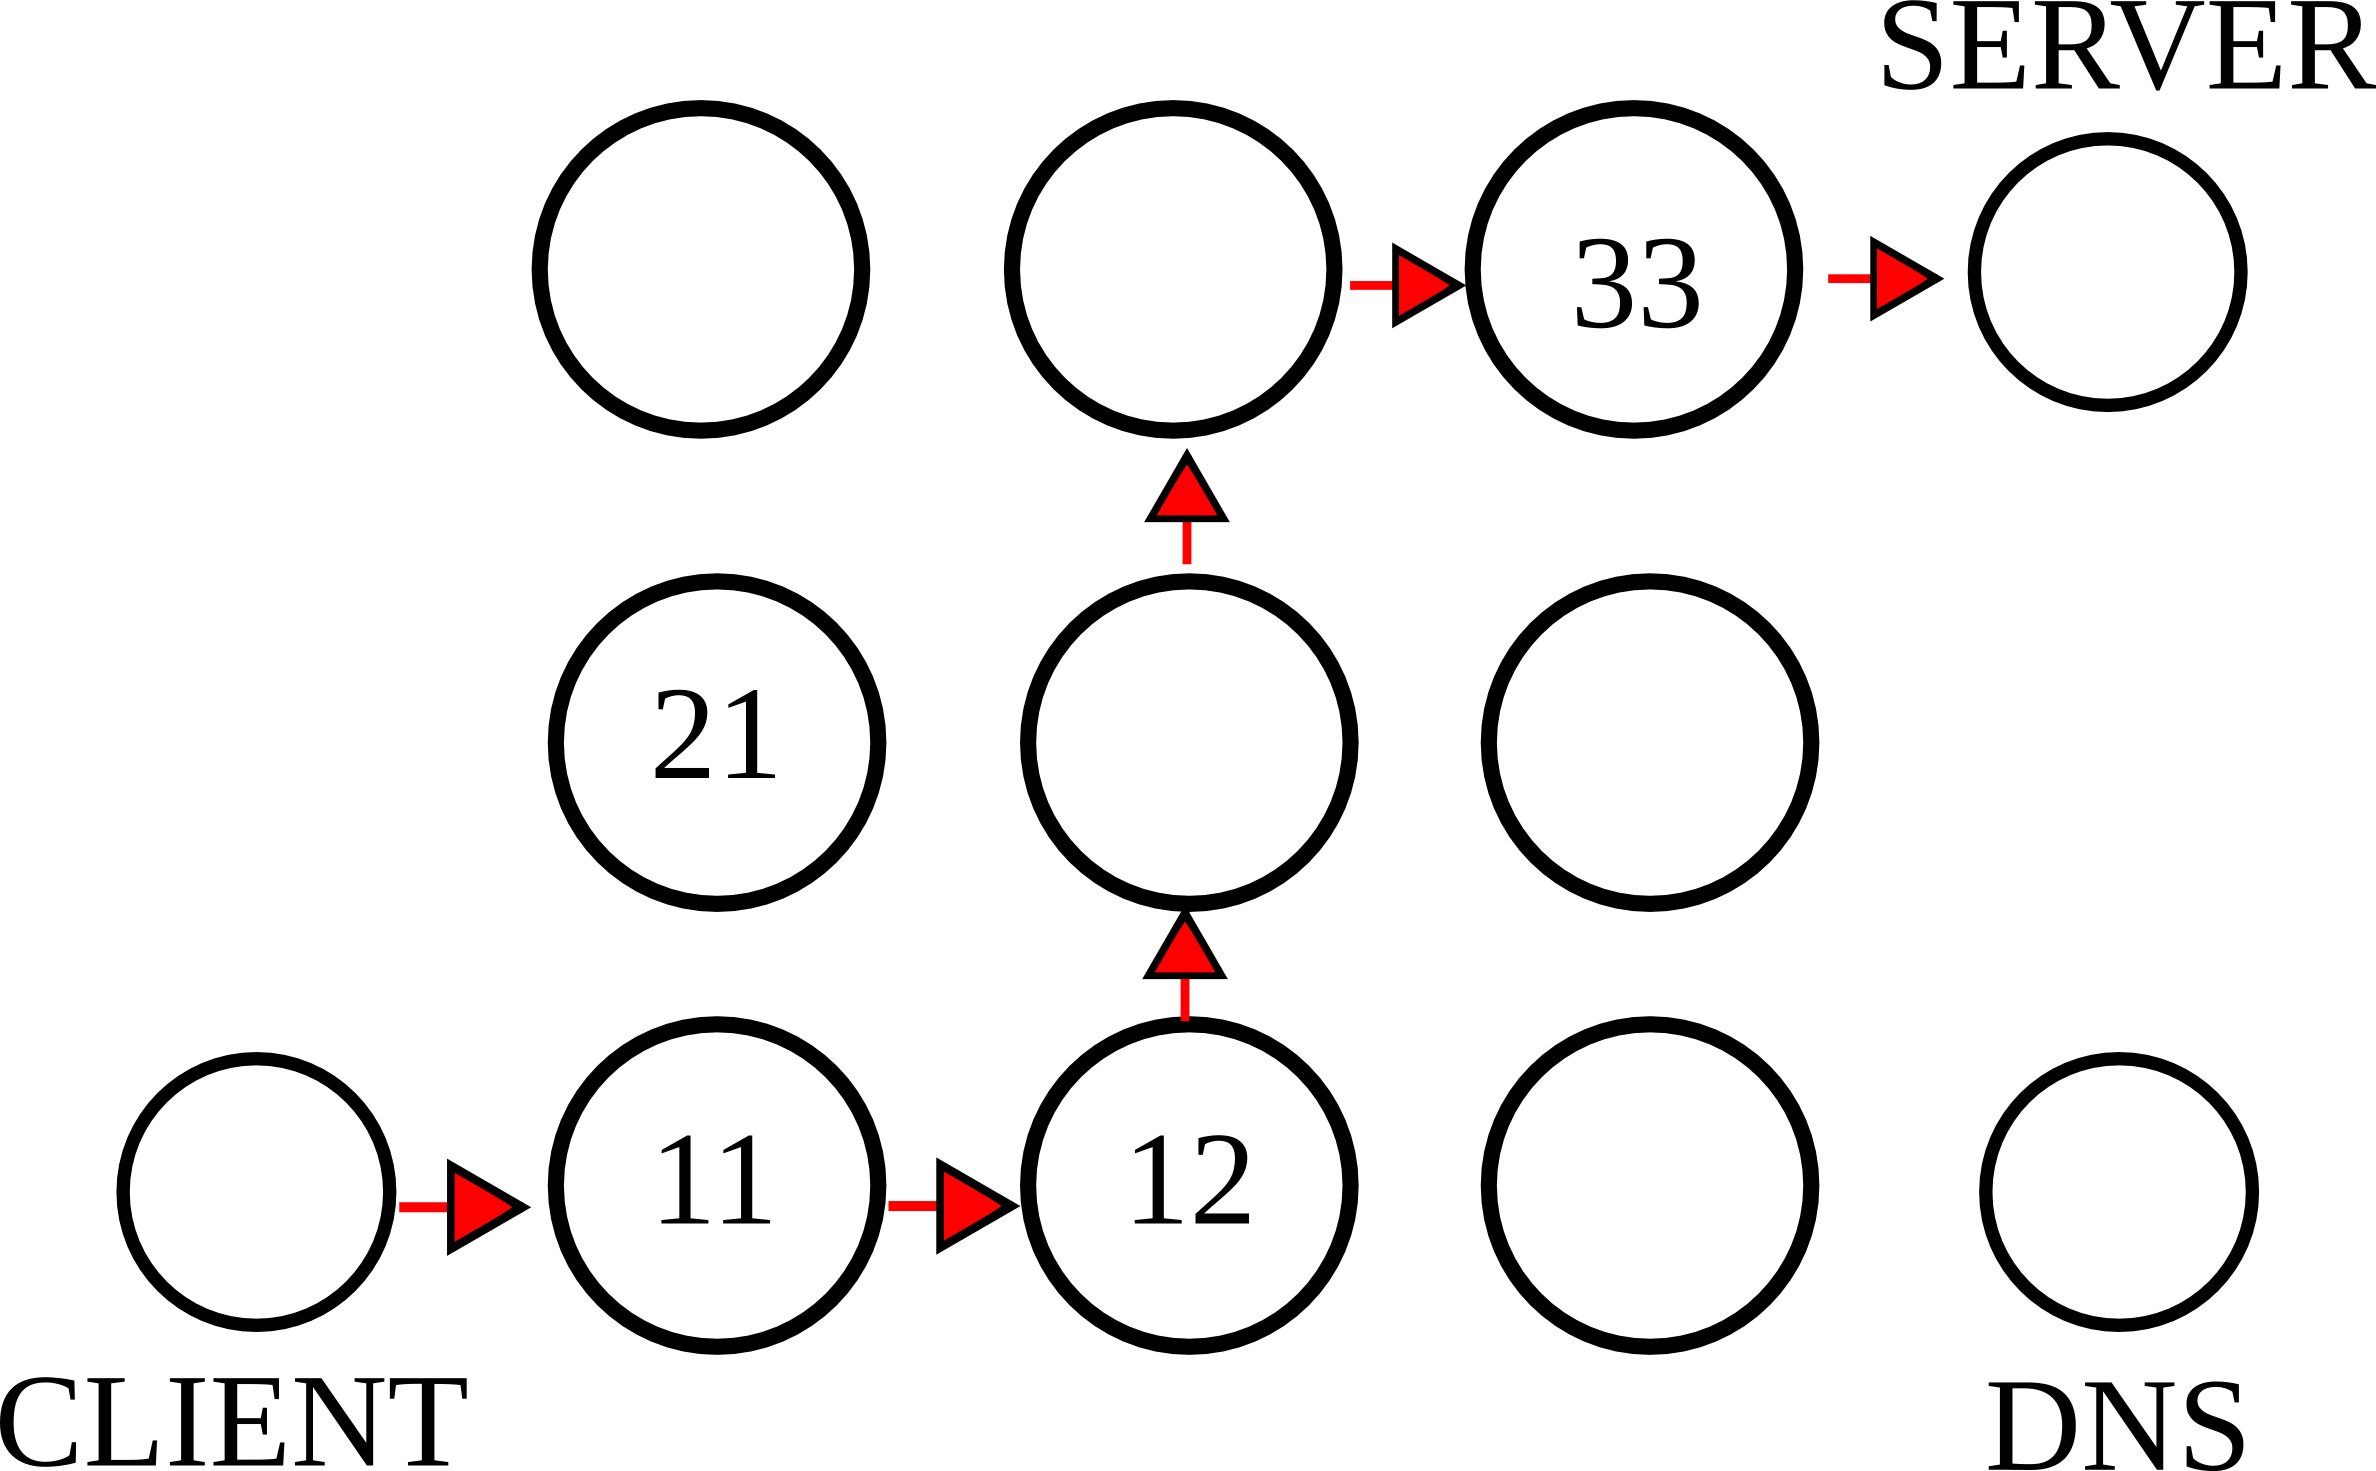
\includegraphics[height=0.7\textheight]{img/kindernet.png}
\end{frame}

\begin{frame}
    \frametitle{Mail}
    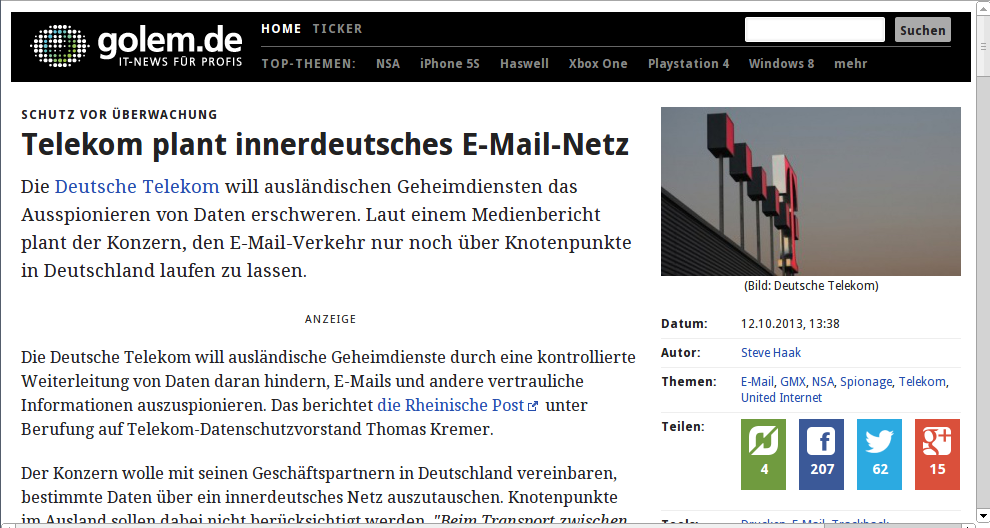
\includegraphics[height=0.7\textheight]{img/telekom_mail.png}
\end{frame}

\begin{frame}
    \frametitle{Verschlüsselung: Analogie}
    \includegraphics[height=0.7\textheight]<2->{img/bote.jpg}
    %\\{\small \href{http://commons.wikimedia.org/wiki/File:Reitbote.jpg}{Grafik}: \href{http://creativecommons.org/licenses/by-sa/2.5/deed.en}{\cc{by-sa}} Ronald Preuss}
\end{frame}

\begin{frame}
    \frametitle{Verschlüsselung: Asymetrische}
    \includegraphics[height=0.7\textheight]<2->{img/asym_encryption.png}
\end{frame}

\begin{frame}
    \frametitle{SSL / TLS}
    \begin{itemize}
      \item<2-> SSL = Secure Socket Layer
      \item<3-> eingesetzt im Web, Mail, ...
      \item<4-> hierarchische Struktur
    \end{itemize}
\end{frame}

\begin{frame}
    \frametitle{SSL im Browser}
    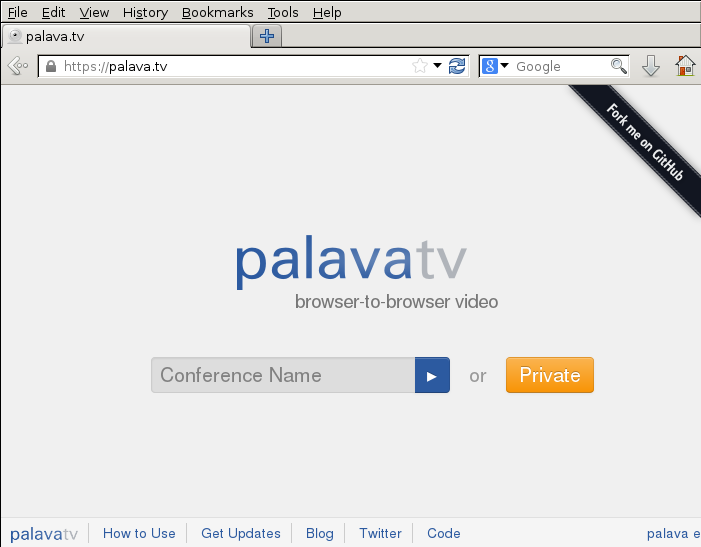
\includegraphics[height=0.7\textheight]{img/ssl_verified.png}
\end{frame}

\begin{frame}
    \frametitle{SSL im Browser}
    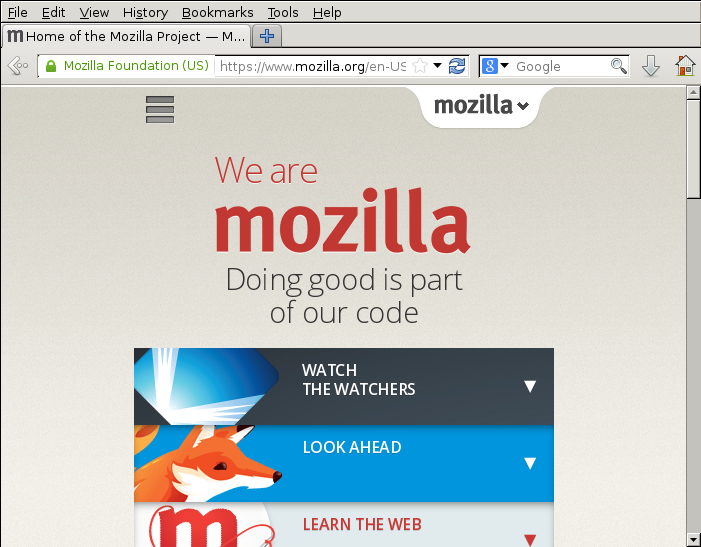
\includegraphics[height=0.7\textheight]{img/ssl_special.png}
\end{frame}

\begin{frame}
    \frametitle{SSL im Browser}
    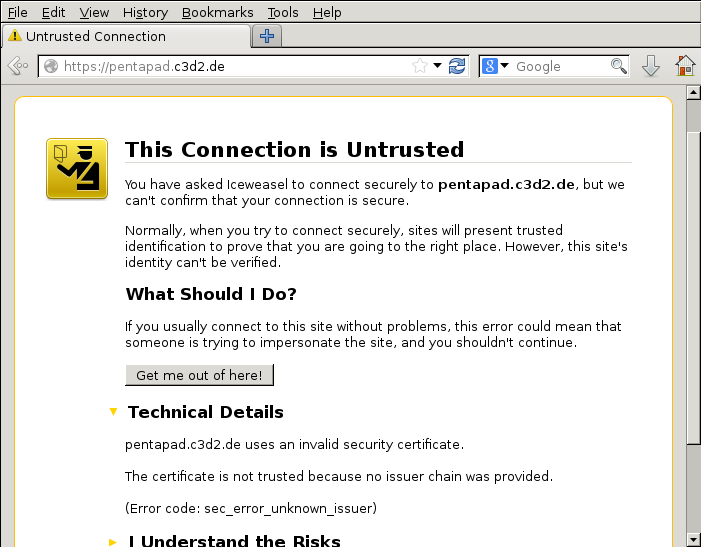
\includegraphics[height=0.7\textheight]{img/ssl_unverified.png}
\end{frame}

\begin{frame}
    \frametitle{Zertifizierungsstellen}
    \begin{center}
      \includegraphics[height=5cm]<2->{img/zertifikate.png}
    \end{center}
\end{frame}

\begin{frame}
  \frametitle{HTTPS Everywhere}
    \begin{center}
      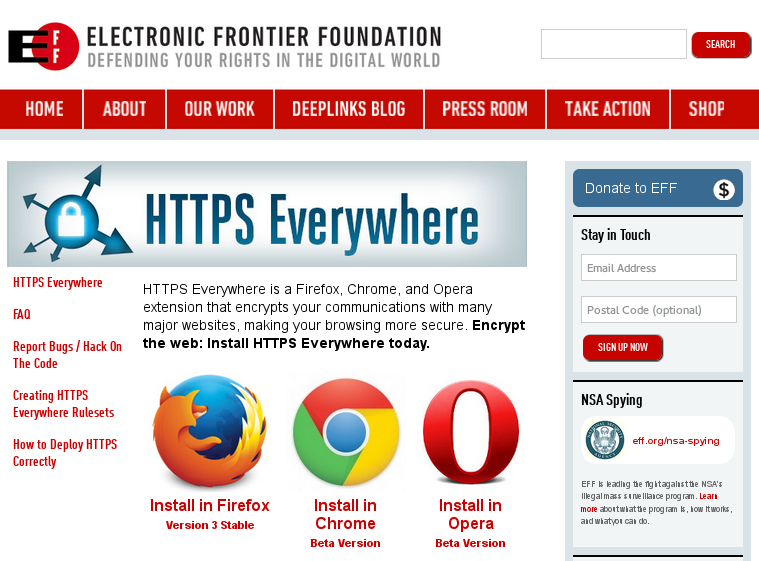
\includegraphics[height=5cm]{img/https-everywhere.png}
    \end{center}
\end{frame}